\newpage

\section{Preliminaries}
\label{sec:appendix-bk}

CoP proposed by~\cite{she2022cop} is calculated based on $\Delta_{p_Y}^{cond}$. Although they only showed $\Delta_{p_Y}^{cond}$ in their paper, they took the logarithm of probabilities during implementation without analysis and explanations. Overall, CoP is:
\begin{equation}
	{\rm CoP} = \frac{1}{m}\sum\nolimits_{i=1}^m \log{p_{y_i}^{s2s}} - \log{p_{y_i}^{pref}}
\end{equation}

HaRiM proposed by~\cite{son2022harim} is derived from $\Delta_{p_Y}^{prior}$:
\begin{equation}
	{\rm HaRiM} = \frac{1}{m}\sum\nolimits_{i=1}^m (1-p_{y_i}^{s2s})[1-({p_{y_i}^{s2s}} - {p_{y_i}^{prior}})]
\end{equation}
Our FFLM is different from HaRiM in three ways: First, we propose to do faithfulness evaluation with foundation language models while they suggested to evaluate with models fine-tuned on summarization data. Second, HaRiM only considers one of the changes with prior probability, i.e., $\Delta_{p_Y}^{prior}$. Our metric not only adds a back constraint of $P(X|Y)$ additionally to HaRiM, but also considers the probability changes with conditional probability. Third,  Specifically for the formula, the intuition of adding weights behind HaRiM and our FFLM are different regardless of the function-form variations. HaRiM's weight $(1-p_{y_i}^{s2s})$ was originally introduced to adjust the loss scale for training better neural machine translation models by~\citet{miao2021prevent}. FFLM adopted the weight $e^{p_{y_i}^{s2s}}$ and the logarithm to pay more attention to low-probability tokens which generally correspond to unfaithful contents according to~\cite{goyal2022training}.

\citet{xie2021factual} introduced another similar metric CoCo which is also based on probability changes. Instead of using the prior probability of $Y$ in $\Delta_{p_Y}^{prior}$ , they condition $Y$ on the masked document $X^\prime$ by removing $Y$-related information. The masking strategy is hard to design since locating the $Y$-related information is uneasy. Their complicated operation also largely slows down the inference speed. 

We compared these three metrics backed on BART for faithfulness ranting in Table~\ref{tab:pilot}. Since CoCo's performances vary a lot with different masking strategies and none of them completely outperform the other two metrics on a single dataset, we didn't compare with it thoroughly in our work.

\begin{table*}[t]
	\scriptsize
	\centering
	\begin{tabular}{l|ccc|ccc|ccc|ccc|ccc}
		\toprule[1pt]
		&  \multicolumn{3}{c}{FRANKCNN} & \multicolumn{3}{c}{QAGSCNN} & \multicolumn{3}{c}{SummEval} & \multicolumn{3}{c}{FRANKXSUM} & \multicolumn{3}{c}{QAGSXSUM} \\
		Metric & $\gamma$ &$\rho$ & $\tau$ & $\gamma$ &$\rho$ & $\tau$ & $\gamma$ &$\rho$ & $\tau$ & $\gamma$ &$\rho$ & $\tau$ & $\gamma$ &$\rho$ & $\tau$ \\
		\hline
		CoP & 56.1 & 51.0 & 39.4 & \textbf{73.0} & \textbf{65.3} & \textbf{53.2} & 23.6 & 22.6 & 18.0 & \textbf{22.8} & \textbf{20.8} & \textbf{17.0} & \textbf{26.6} & 25.3 & 20.7 \\
		HaRiM & \textbf{61.0} & 53.9 & 42.1 & 67.4 & 58.2 & 47.1 & \textbf{42.7} & \textbf{37.6} & \textbf{29.8} & 14.8 & 13.9 & 11.4 & 15.8 & 16.0 & 13.1 \\ 
		CoCo$_{\rm token}$ & 55.9 & 50.1 & 39.0 & 64.7 & 53.1 & 42.6 & 41.3 & 36.8 & 29.1 & 8.0 & 6.8 & 5.6 & 21.4 & 22.8 & 18.7 \\
		CoCo$_{\rm span}$ & 56.9 & 50.3 & 39.1 & 66.4 & 56.0 & 45.0 & 39.5 & 35.3 & 27.9 & 12.7 & 11.8 & 9.6 & 25.3 & \textbf{26.1} & \textbf{21.4} \\
		CoCo$_{\rm sent}$ & 60.9 & \textbf{54.1} & \textbf{42.2} & 71.7 & 62.0 & 50.2 & 39.4 & 35.0 & 27.6 & 16.3 & 15.8 & 12.9 & 16.5 & 14.9 & 12.2\\
		CoCo$_{\rm doc}$ & 59.9 & 54.0 & 42.1 & 71.6 & 61.9 & 50.2 & 39.1 & 34.8 & 27.5 & 18.5 & 17.2 & 14.1 & 22.1 & 21.5 & 17.6 \\
		\bottomrule[1pt]
	\end{tabular}
	\caption{Correlations(\%) of comparisons among CoP, HaRiM, and CoCo with BART for faithfulness rating. The highest scores are in bold.} % add the similar table for summac in appendix
	\label{tab:pilot}
\end{table*}

\begin{table*}[t]
	\scriptsize
	\centering
	\begin{tabular}{l|cccccc}
		\toprule[1pt]
		Metric & CoGenSum & SummEval & FRANK & Polytope & FactCC & XSumFaith \\
		\hline
		FFLM & \textbf{71.8} & \textbf{83.9} & \textbf{84.4} & 61.5 & 77.3 & {58.9} \\
		\hline
		\multicolumn{7}{l}{\textit{Ablations on the metric components }}\\
		$\Delta_Y^{prior}$ & 52.2 & 64.6 & 76.2 & 54.8 & 55.8 & \textbf{60.5} \\
		$\Delta_X^{prior}$ &49.5 & 67.9 & 73.4 & 62.0 & 55.4 & 58.6 \\
		
		$\Delta_Y^{cond}$ & 64.4 & 82.9 & 83.1 & 56.8 & 79.0 & 53.5\\
		
		$\Delta_Y^{prior}$, $\Delta_X^{prior}$&  54.7 & 65.6 & 77.4 & 62.0 & 55.0 & 58.9  \\
		$\Delta_Y^{prior}$, $\Delta_Y^{cond}$ & 70.5 & 83.5 & \textbf{84.4} & 56.8 & 77.3 & {59.8}\\
		$\Delta_X^{prior}$, $\Delta_Y^{cond}$ &  64.4 & 83.5 & 83.6 & 61.5 & 78.6 & 58.6 \\ 
		
		\hline
		\multicolumn{7}{l}{\textit{Ablations on the metric design}} \\
		- w/o $w$ & 69.5 & 83.3 & 83.5 & \textbf{66.7} & \textbf{77.4} & 57.8  \\
		- w/o $\log$ &68.7 & 78.5 & 83.5 & 60.9 & 74.2 & 58.1 \\
		- w/o $w$ and $\log$ & 65.3 & 80.9 & 83.1 & 64.1 & 75.2 & 56.6 \\
		
		
		\bottomrule[1pt]
	\end{tabular}
	\caption{Ablations of FFLM for inconsistency detection. The highest scores are in bold.} 
	\label{tab:ablation-id}
\end{table*}



\begin{table*}[h!]
	\scriptsize
	\centering
	\begin{tabular}{l|cccccc}
		\toprule[1pt]
		Metric & CoGenSum & SummEval & FRANK & Polytope & FactCC & XSumFaith \\
		
		\hline
		\multicolumn{7}{l}{\textit{Prompting Approach}} \\
		LLaMa-7b &  54.3 & 50.0 & 53.6 & 53.7 & 51.7 & 51.7 \\
		Vicuna-7b & 56.9 & \underline{58.1} & \underline{69.2} & \underline{54.6} & \underline{69.0} & \underline{55.5}\\
		Alpaca-7b & \underline{57.8} & 50.0 & 57.5 & 52.6 & 58.8 & 51.1 \\
		\hline
		\multicolumn{7}{l}{\textit{Our Approach}} \\
		LLaMa-7b &  \underline{\textbf{71.8}} & 83.9 & \underline{\textbf{84.4}} & \underline{\textbf{61.5}} & 77.3 & 58.9 \\
		Vicuna-7b & 68.6 & 83.2 & 83.8 & 58.3 & 77.2 & 58.9 \\
		Alpaca-7b & 65.2 & \underline{\textbf{85.0}} & 83.9 & 59.1 & \underline{\textbf{78.5}} & \underline{\textbf{60.7}} \\
		\bottomrule[1pt]
	\end{tabular}
	\caption{Comparisons with prompting and instruction-tuning techniques under the same model size for inconsistency detection. The highest scores are in bold in each column and are underlined among each kind of approach.}
	\label{tab:prompt-id}
\end{table*}


\section{Analysis on Inconsistency Detection}
\label{sec:appendix}

Ablation studies of FFLM for inconsistency detection are in Table~\ref{tab:ablation-id}. 
Fig.~\ref{fig:sizes-id} illustrates the performances of FFLM on variable sizes of the foundation language model.
Results with the prompting approach and comparison to the instruction-tuning technique are in Table~\ref{tab:prompt-id}.




\begin{figure}[th]
	\centering
	\begin{minipage}[t]{\linewidth}
		\centering
		\subfloat{
			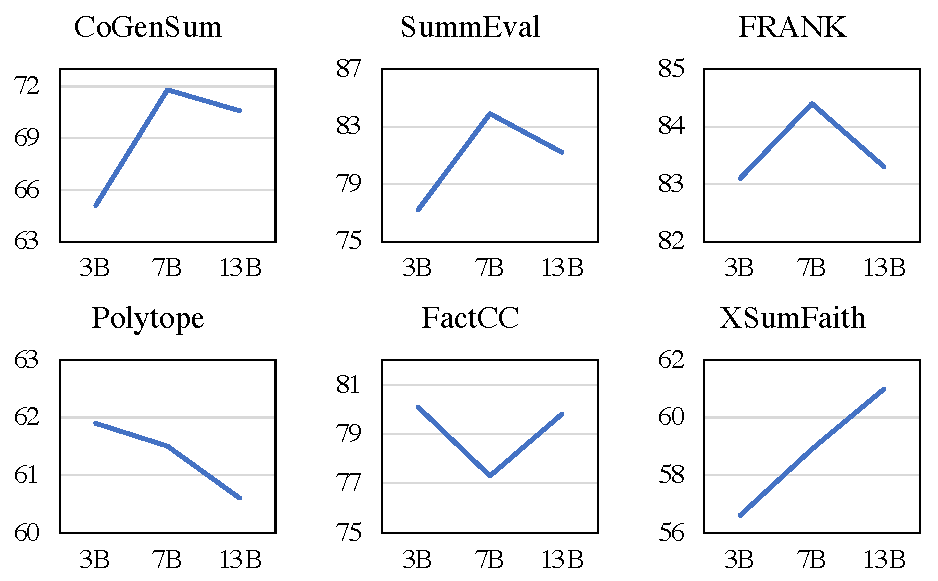
\includegraphics[scale=0.4]{sizes-id.pdf}
			%\caption{fig1}
		}%
	\end{minipage}%
	
	\caption{Spearman correlation(\%) of FFLM with different model sizes on inconsistency detection datasets.}
	\label{fig:sizes-id}
\end{figure}


The observations for inconsistency detection are in line with those for faithfulness ranting. Another finding is that the gap between prompting approaches and FFLM under this setup is much smaller than that under the faithfulness rating setup.
This indicates that inconsistency detection is easier than faithfulness rating with less number of answer choices when doing faithfulness evaluation by prompting large models.



%\begin{table*}[h]
%	\scriptsize
%	\centering
%	\begin{tabular}{l|cccccc}
%		\toprule[1pt]
%			& CoGenSum & SummEval & FRANK & Polytope & FactCC & XSumFaith \\

%		\hline
%		3b & 65.1 & 77.2 & 83.1 & \textbf{61.9} & \textbf{80.1} & 56.6\\
%		7b & \textbf{71.8} & \textbf{83.9} & \textbf{84.4} & 61.5 & 77.3 & 58.9 \\
%		13b & 70.6 & 81.2 & 83.3 & 60.6 & 79.8 & \textbf{61.0}\\
%		\bottomrule[1pt]
%	\end{tabular}
%	\caption{FFLM with different sizes of LLaMa for inconsistency detection.} 
%	\label{tab:modelsizes-id}
%\end{table*}




\section{A Collection of Prompts}
\label{sec:appendix-prompt}

The prompts we collected are in Table~\ref{tab:prompt-templates}. We made tiny changes to some of the prompts to enhance their probability of generating an acceptable answer, such as adding a hint like "Marks:" and moving the answer choices to the end of the prompt.
We recognize the faithfulness score by analyzing the generations with simple rules. If there isn't an acceptable answer, we regard the summary as unfaithful, i.e., ``No'' for inconsistency detection and ``1'' for faithfulness rating.

\begin{table}[h!]
	\scriptsize
	\centering
	\begin{tabular}{l|p{4.85cm}}
		\toprule[1pt]
		 Citation & Prompt \\
		\hline
		\multicolumn{2}{l}{\textit{Inconsistency Detection}} \\
		 \citet{chen2023evaluating} &\makecell[l]{\{Document\} \\Q: Can the following statement be inferred from \\the above document? Yes or No?\\\{Summary\}\\A:} \\
		\hline
		  \citet{gao2023human} &\makecell[l]{Is the sentence supported by the article?\\Article: \{Document\}\\Sentence: \{Summary\}\\Answer "Yes" or "No":} \\
		\hline
		\citet{luo2023chatgpt} & \makecell[l]{Decide if the following summary is consistent with \\the corresponding article.\\Article: \{Document\}\\Summary: \{Summary\}\\Answer (yes or no):} \\
		\hline
		
		\multicolumn{2}{l}{\textit{Faithfulness Rating}} \\
		 \citet{gao2023human} & \makecell[l]{Evaluate the quality of summaries written for a \\news article. Rate each summary on consistency. \\You should rate on a scale from 1 (worst) to 5 \\(best).\\Article: \{Document\}\\Summary: \{Summary\}\\Marks:} \\
		\hline
	 \citet{luo2023chatgpt} & \makecell[l]{Score the following summary given the \\corresponding article with respect to consistency \\from 1 to 10. Note that consistency measures how\\ much information included in the summary is \\present in the source article. 10 points indicate the \\summary contains only statements that are entailed \\by the source document.\\Summary: \{Summary\}\\ Source Article: \{Document\}\\Marks:} \\
		\bottomrule[1pt]
	\end{tabular}
	\caption{A collection of prompts.``\{\}'' marks placeholders for corresponding contents.}
	\label{tab:prompt-templates}
\end{table}


\section{Performance of Different Prompts}
\label{sec:diff-prompts}

We show the performances of different prompts with Vicuna-7B for inconsistency detection in Table~\ref{tab:vicuna-prompt-id} and for faithfulness rating in Table~\ref{tab:vicuna-prompt-fr}. The performance with different prompts for the same task varies a lot. And some prompts used in previous works with ChatGPT failed with smaller models, showing the high-level language understanding and generation ability requirements for prompting large language models. 


\begin{table}[t]
	\scriptsize
	\centering
	\begin{tabular}{l|ccc}
		\toprule[1pt]
		Dataset & \citet{chen2023evaluating} & \citet{gao2023human} & 	\citet{luo2023chatgpt}  \\
		\hline
		CoGenSum & \textbf{56.9} & 49.8 & 49.4 \\
		SummEval & \textbf{58.1} & 50.2 & 54.5 \\
		FRANK & \textbf{69.2}  & 46.9 & 57.8 \\
	Polytope	& \textbf{54.6} & 51.0 & 52.8 \\
	FactCC & \textbf{69.0} & 51.7 & 53.8 \\
	XSumFaith & 52.2 & 49.6 & \textbf{55.5} \\
		
	%	& CoGenSum & SummEval & FRANK & Polytope & FactCC & XSumFaith \\
	%	\hline
	%	\citet{chen2023evaluating} & \textbf{56.9} & \textbf{58.1} & \textbf{69.2} & \textbf{54.6}& \textbf{69.0} & 52.2 \\
	%	\citet{gao2023human} & 49.8 & 50.2 & 46.9 & 51.0& 51.7 & 49.6\\
	%		\citet{luo2023chatgpt} & 49.4 &  54.5 & 57.8 & 52.8 & 53.8 & \textbf{55.5}\\
		
		\bottomrule[1pt]
	\end{tabular}
	\caption{Balanced accuracy(\%) of Vicuna-7B with different prompts for inconsistency detection. The highest accuracy on each dataset is in bold.} 
	\label{tab:vicuna-prompt-id}
\end{table}

\begin{table}[t]
	\scriptsize
	\centering
	\begin{tabular}{l|cc}
		\toprule[1pt]
		Dataset & 	\citet{gao2023human} & \citet{luo2023chatgpt}\\
		\hline
		FRANKCNN & \textbf{17.4} & -5.0 \\
		QAGSCNN & \textbf{19.8} & 4.6 \\
		SummEval & \textbf{11.9} & -0.9 \\
		FRANKXSUM &\textbf{5.5} & -3.6 \\
		QAGSXSUM & \textbf{8.4} & -3.3 \\
		
	%	& FRANKCNN & QAGSCNN & SummEval & FRANKXSUM & QAGSXSUM \\
	%	\hline
	%	\citet{gao2023human}  & 17.4 & 19.8 & 11.9 & 5.5 & 8.4\\
	%	 \citet{luo2023chatgpt}  & -5.0 & 4.6 & -0.9 & -3.6 & -3.3\\
		
		\bottomrule[1pt]
	\end{tabular}
	\caption{Spearman correlation(\%) of Vicuna-7B with different prompts for faithfulness rating. The highest correlation on each dataset is in bold.} 
	\label{tab:vicuna-prompt-fr}
\end{table}